\addtocontents{toc}{\vspace{\baselineskip}\noindent{\titlefont\bfseries\large II\quad State of the Art}\par\vspace{0.3em}}
\chapter{Classical Approaches in RTS Games}
\label{chap:historical-approach}

This chapter reviews three classical paradigms for RTS AI: rule-based, search-based, and hierarchical. Each is illustrated with agents from the MicroRTS competition, drawn from the evaluation benchmark assembled in Chapter~\ref{chap:evaluation-framework}. Figure~\ref{fig:paradigm-progression} arranges them in the chronological order of their introduction in game AI: each emerged to address limitations of existing approaches by integrating new mechanisms~\cite{robertsonReviewRealTimeStrategy2014, ontanonRTSAIProblems2015}. Newer paradigms, however, have not displaced older ones; all three remain in active use today and are routinely combined within single systems~\cite{barrigaImprovingRTSGame2019}, as exemplified by AlphaZero, which combines DRL with search~\cite{silverMasteringChessShogi2017}. Whether used in isolation or in combination, their shared reliance on hand-designed control motivates the transition to DRL (Chapter~\ref{chap:sota}).

\begin{figure}[ht]
\centering
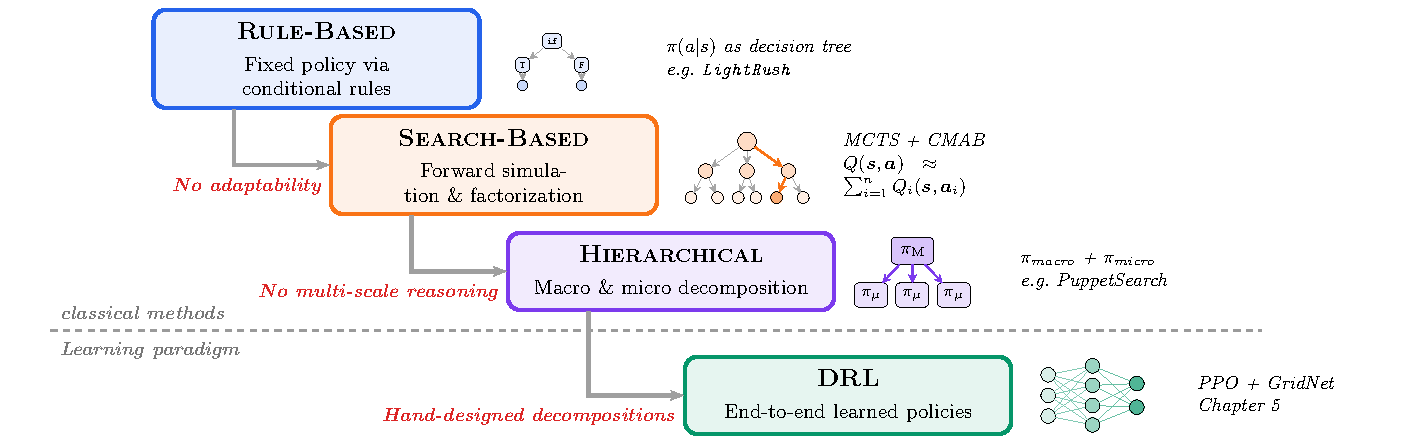
\includegraphics[width=\textwidth]{chapters/04_classical_approaches_rts/figures/paradigm_progression.pdf}
\caption[AI paradigms for RTS games]{AI paradigms for RTS games in chronological order of introduction, from fixed conditional rules to end-to-end learned policies. Each addresses limitations of earlier ones without displacement.}
\label{fig:paradigm-progression}
\end{figure}

\vspace{-1.8em}

\section{Rule-Based Approaches}
\label{sec:rule-based}

A common classical approach to RTS game AI is rule-based control, which encodes a fixed policy $\pi(a|s)$ through manually designed conditional rules~\cite{sweetserCurrentAIGames2002}. Each unit's action is selected by traversing a priority-ordered decision tree over the game state, without learning or search.

\begin{lstlisting}[
caption={Pseudocode of a simplified \code{LightRush} policy in MicroRTS.},
label={lst:rush-bot}
]
for unit in my_units:
    if is_type(unit, Base):
        if count(Worker) < 2 and resources >= 1:
            train(Worker)
        elif not exists(Barracks) and resources >= 5:
            build(Barracks, adjacent_pos)
    elif is_type(unit, Barracks):
        if resources >= 2:
            train(Light)
    elif (is_type(unit, Light) or is_type(unit, Worker)) and is_idle(unit):
        enemy = nearest_enemy(unit)
        if enemy and in_attack_range(unit, enemy):
            attack(unit, enemy)
        else:
            move_toward(unit, enemy_base)
\end{lstlisting}

Listing~\ref{lst:rush-bot} illustrates this structure with a simplified \code{LightRush} strategy. The policy is entirely defined by three conditional blocks: the base produces up to two Workers before constructing a Barracks; the Barracks then trains Light units; and any idle unit (Workers included) either attacks an enemy in range or advances toward the opponent's base.

Despite this simplicity, rule-based agents remain competitive in MicroRTS competitions: hand-tuned heuristics are highly effective in anticipated scenarios, while full interpretability and low computational cost make them attractive baselines.

Strong examples from recent editions include the following: \urlref{https://github.com/Coac/coac-ai-microrts}{\emph{CoacAI}} ($2020$) uses heuristic economy management with $A^{*}$ pathfinding; \urlref{https://github.com/barvazkrav/mayariBot}{\emph{Mayari}} ($2021$) performs greedy per-action heuristic scoring with local distance estimation; \urlref{https://github.com/Jannis42/MicroRTSObiBotKenobi}{\emph{ObiBotKenobi}} ($2023$) combines unit-role assignment with Dijkstra-based pathfinding; \urlref{https://github.com/MazzaAlessandro/TMA}{\emph{TMA}} ($2024$) selects between four strategy combinations (attack/defense $\times$ worker/military), recalibrated every $500$ game cycles.

However, rule-based policies adapt only within the scenarios 
anticipated by their hand-designed rules, with no mechanism to improve from experience. This motivated search-based approaches that adapt behavior to novel states through forward simulation.

\section{Search-Based Approaches}
\label{sec:search-based}

Search-based approaches derive actions through explicit forward simulation of future consequences. Classical methods such as Minimax with Alpha-Beta pruning~\cite{shannonXXIIProgrammingComputer1950, knuthAnalysisAlphabetaPruning1975} defined the early state of the art in turn-based games, culminating in IBM Deep Blue's $1997$ defeat of world chess champion Garry Kasparov~\cite{campbellDeepBlue2002}. A real-time variant, Iterative Deepening Real-Time Minimax (IDRTMinimax), adapts this to RTS games by searching as deep as possible within a fixed time budget~\cite{ontanonExperimentsGameTree2012}. However, feasibility depends critically on the \emph{joint} branching factor $b$ (legal actions per state, taken jointly over all controlled units): for a search depth $d$, the number of nodes grows as $O(b^d)$. Figure~\ref{fig:branching-factor} compares branching factors across board and RTS games.

\begin{figure}[htbp]
  \centering
  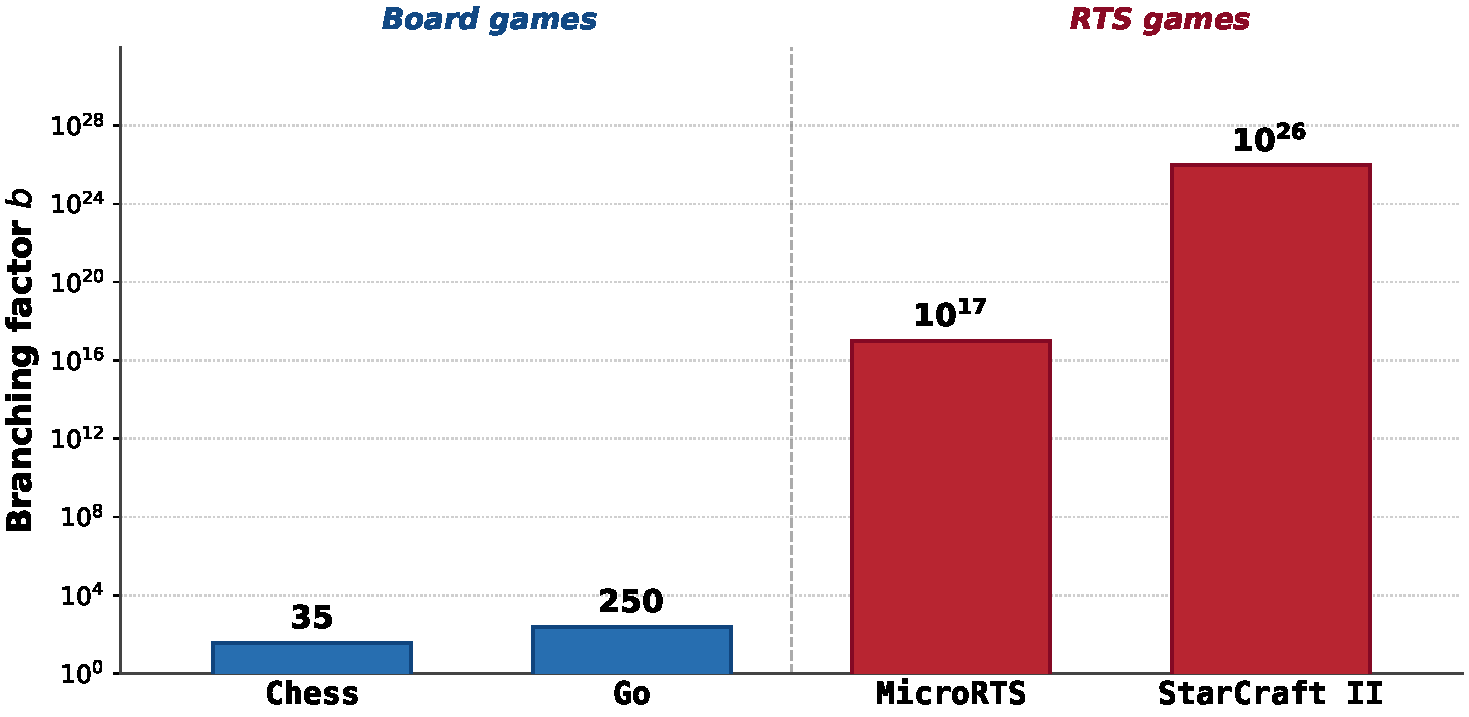
\includegraphics[width=0.7\textwidth]{chapters/04_classical_approaches_rts/figures/branching_factors.pdf}
  \caption[Branching factors across board and RTS games]{Branching factor estimates across board and RTS games. Board game values from~\cite{silverMasteringGameGo2016}; MicroRTS value is the average on a $12{\times}12$ map with $4$ starting bases~\cite{ontanonCombinatorialMultiarmedBandits2017}; StarCraft~II from~\cite{vinyalsGrandmasterLevelStarCraft2019}. RTS values should be interpreted as order-of-magnitude estimates, since the branching factor depends strongly on the state, map, unit count, and action abstraction used.}
  \label{fig:branching-factor}
\end{figure}

Branching factors for RTS games exceed even Go's by several orders of magnitude. Despite aggressive pruning, they render exhaustive search infeasible under real-time constraints~\cite{ontanonCombinatorialMultiarmedBandits2017}.

\subsection{Monte Carlo Tree Search}

Monte Carlo Tree Search (MCTS) replaces exhaustive enumeration with stochastic sampling~\cite{browneSurveyMonteCarlo2012, swiechowskiMonteCarloTree2023, chaslotPROGRESSIVESTRATEGIESMONTECARLO2008}. It estimates action values $Q(s,a)$ by averaging returns over rollouts. A key property is its \emph{anytime behavior}: it can return a decision at any point, with quality improving as more simulations complete. MCTS is best known as the core algorithm of AlphaGo~\cite{silverMasteringGameGo2016}, discussed in Chapter~\ref{chap:sota}.

However, standard MCTS remains insufficient for RTS environments: the exponential joint action space means most actions are never sampled, and the sparse terminal rewards typical of RTS games provide minimal guidance during rollouts. \urlref{https://github.com/zuozhiyang/Droplet}{\emph{Droplet}} ($2019$) targets the action-space problem through script-biased sampling that steers MCTS toward promising action sequences, but the combinatorial explosion ultimately remains. This motivates approaches that explicitly factorize the action space.

\subsection{Combinatorial Multi-Armed Bandits}

Combinatorial Multi-Armed Bandits (CMAB)~\cite{ontanonCombinatorialMultiarmedBandits2017} address the combinatorial explosion of the action space through factorization, approximating the joint action-value function as:
\begin{equation}
Q(\boldsymbol{s}, \boldsymbol{a}) \approx \sum_{i=1}^n Q_i(\boldsymbol{s}, \boldsymbol{a}_i),
\label{eq:cmab}
\end{equation}
where $Q_i(\boldsymbol{s}, \boldsymbol{a}_i)$ estimates the contribution of unit $i$'s action to the global reward. This relies on an \emph{independence assumption}: actions are assumed to have limited cross-dependencies (e.g., units on opposite sides of the map act independently). Under this independence, the number of values to estimate drops from $O(k^n)$ joint-action values to $O(nk)$ per-unit action values, where $k$ counts actions per unit, enabling tractable planning even with dozens of units (Figure~\ref{fig:cmab-factorization}).

\begin{figure}[ht]
\centering
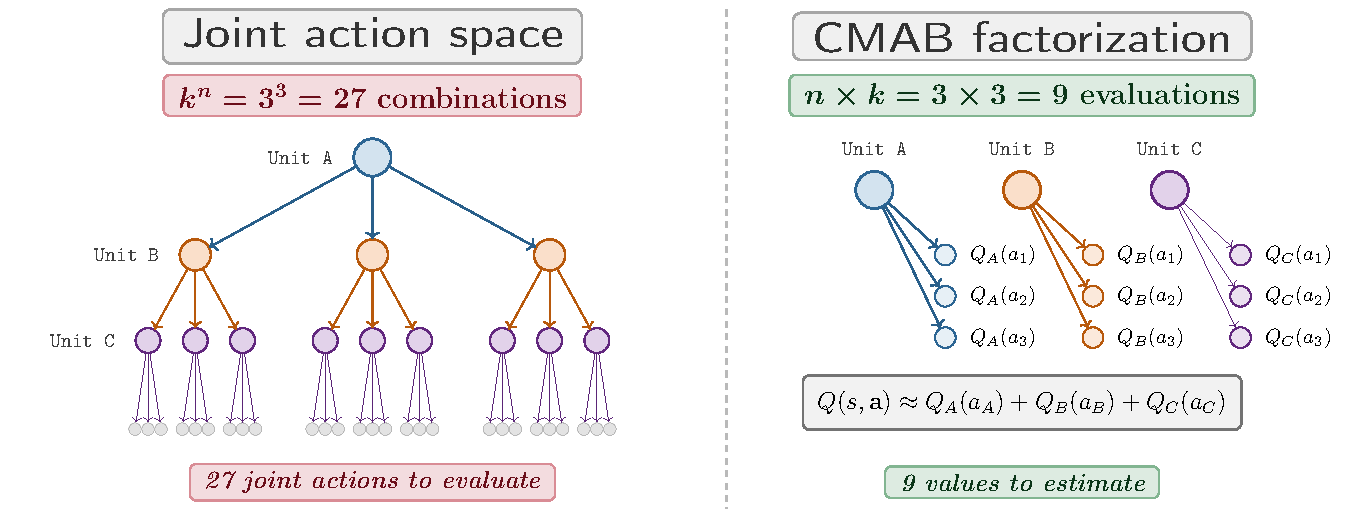
\includegraphics[width=\textwidth]{chapters/04_classical_approaches_rts/figures/cmab_factorization.pdf}
\caption[Joint action space vs CMAB factorization]{Joint action space vs CMAB factorization (3 units, 3 actions each). Left: $k^n$ joint evaluations. Right: $nk$ per-unit evaluations under the independence assumption (Equation~\ref{eq:cmab}).}
\label{fig:cmab-factorization}
\end{figure}

NaïveMCTS~\cite{ontanonCombinatorialMultiarmedBandits2017} combines CMAB with MCTS by estimating per-unit $Q_i$ values during the tree search. The Informed variant~\cite{ontanonInformedMonteCarlo2016} additionally guides rollouts using handcrafted strategies such as \code{LightRush} (Listing~\ref{lst:rush-bot}). Further gains were achieved by grouping unit commands into higher-level action abstractions~\cite{moraesActionAbstractionsCombinatorial2018, marinoEvolvingActionAbstractions2019}.

Despite substantial gains over standard MCTS, CMAB remains constrained by limited search horizons and the independence assumption, which breaks down when units must coordinate closely. This factorization principle reappears in Chapter~\ref{chap:sota}, where GridNet (a spatial neural network architecture) applies the same independence assumption to neural network outputs, producing per-cell action distributions $\pi_\theta(\boldsymbol{a}_i | \boldsymbol{s})$ rather than estimating $Q_i$ through search.

Beyond the independence assumption, CMAB treats all decisions at a single temporal scale, conflating strategy with tactics. Hierarchical approaches address this temporal limitation.

\section{Hierarchical Approaches}
\label{sec:hierarchical}

As introduced in Section~\ref{sec:rts}, RTS games require decisions at two scales: macro-management (economy, production) and micro-management (unit control, combat). Rule-based and search-based methods treat both scales uniformly. Hierarchical approaches instead decompose the policy $\pi(a|s)$ into specialized components for each level, as illustrated in Figure~\ref{fig:hierarchical}. Table~\ref{tab:macro-micro} lists representative techniques from the literature at each scale.

\begin{figure}[!ht]
\centering
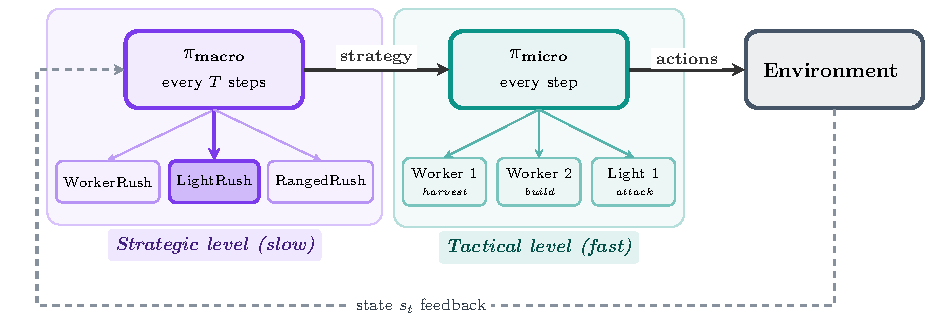
\includegraphics[width=\textwidth]{chapters/04_classical_approaches_rts/figures/hierarchical_decomposition.pdf}
\caption[Hierarchical decomposition (StrategyTactics)]{Hierarchical decomposition illustrated with \urlref{https://github.com/nbarriga/microRTSbot}{StrategyTactics} ($2017$)~\cite{barrigaCombiningStrategicLearning2017, barrigaGameTreeSearch2018}: $\pi_{\text{macro}}$ periodically selects a strategy; $\pi_{\text{micro}}$ translates it into per-unit actions every step.}
\label{fig:hierarchical}
\end{figure}

\vspace{-1.5em}

\begin{table}[!ht]
\centering
\caption[Representative techniques by decision scale in classical RTS AI]{Representative techniques used at each decision scale in classical RTS AI.}
\label{tab:macro-micro}
\small
\begin{tabularx}{\textwidth}{l X}
\toprule
\textbf{Technique} & \textbf{Description} \\
\midrule
\multicolumn{2}{l}{\textit{Macro-management}} \\
\midrule
Hierarchical Task Networks & Decompose strategic goals into ordered subtasks~\cite{ontanonAHTN2015} \\
Bayesian Opponent Modeling & Infer opponent strategy to adapt plans~\cite{synnaeveBayesianModelPlan2011} \\
Goal-Driven Autonomy & Detect expectation failures and reformulate goals~\cite{weberApplyingGoalDrivenAutonomy2010} \\
\midrule
\multicolumn{2}{l}{\textit{Micro-management}} \\
\midrule
Potential Fields & Compute attractive and repulsive forces for unit positioning~\cite{hagelbackRisePotentialFields2008} \\
Behavior Trees & Provide modular structures for reactive unit control~\cite{robertsonBuildingBehaviorTrees2015} \\
Neuroevolution & Evolve neural network controllers for micromanagement~\cite{gajurelNeuroevolutionRTSMicro2018} \\
\bottomrule
\end{tabularx}
\end{table}

MicroRTS competition agents following similar hierarchical designs include \urlref{https://github.com/jr9Hernandez/TiamatBot}{\emph{Tiamat}} ($2018$), which combines evolved action abstractions with online strategy-tactics search; \urlref{https://github.com/AmoyZhp/MixedBotmRTS}{\emph{MixedBot}} ($2019$), which extends Tiamat's strategic search with CMAB-based tactical execution and dynamic time allocation; and \urlref{https://github.com/narsue/UTS_Imass}{\emph{UtsImass}} ($2019$), which tunes build parameters~\cite{churchillBuildOrderOptimization2011} via pre-game self-play before switching to rule-based control with Jump Point Search (JPS)~\cite{haraborOnlineGraphPruning2011}, an optimized A$^*$ variant for grid pathfinding.

\paragraph*{From Classical Methods to DRL.}
All paradigms reviewed in this chapter share a common limitation: their effectiveness rests on hand-designed components that the designer must specify in advance~\cite{ontanonRTSAIProblems2015, adilStateoftheArtOpenChallenges2017}. Figure~\ref{fig:paradigm-progression} positions DRL as a different paradigm: by learning parts of the policy and representation from experience, DRL reduces the need for hand-designed decision rules, although environment design, action abstractions, rewards, and architectures remain important engineering choices. Design effort thus shifts from encoding behavior directly to specifying the conditions under which behavior can be learned.